\begin{tikzpicture}
  \creategridjps{9}{7}
%  \drawobstaclejps{2}{8}
%  \draw[->] (0.7,2.7) -- (1.3,3.3);
  \drawgridnodejps{4}{5}{$N$}
  \drawobstaclejps{7}{7}
  \drawobstaclejps{8}{4}
  \drawobstaclejps{8}{3}
  \drawgridnodejps{2}{7}{$1$}
  \draw[->] (3.3,4.7) -- (1.7,6.3);
  \drawgridnodejps{4}{7}{$2$}
  \draw[->] (3.5,4.7) -- (3.5,6.3);
  \drawgridnodejps{5}{6}{$3$}
  \draw[->] (3.7,4.7) -- (4.3,5.3);
  \drawgridnodejps{8}{5}{$4$}
  \draw[->] (3.7,4.5) -- (7.3,4.5);
  \drawgridnodejps{7}{2}{$5$}
  \draw[->] (3.7,4.3) -- (6.3,1.7);
  \drawgridnodejps{4}{1}{$6$}
  \draw[->] (3.5,4.3) -- (3.5,0.7);
  \drawgridnodejps{1}{2}{$7$}
  \draw[->] (3.3,4.3) -- (0.7,1.7);
  \drawgridnodejps{1}{5}{$8$}
  \draw[->] (3.3,4.5) -- (0.7,4.5);
\end{tikzpicture} \qquad
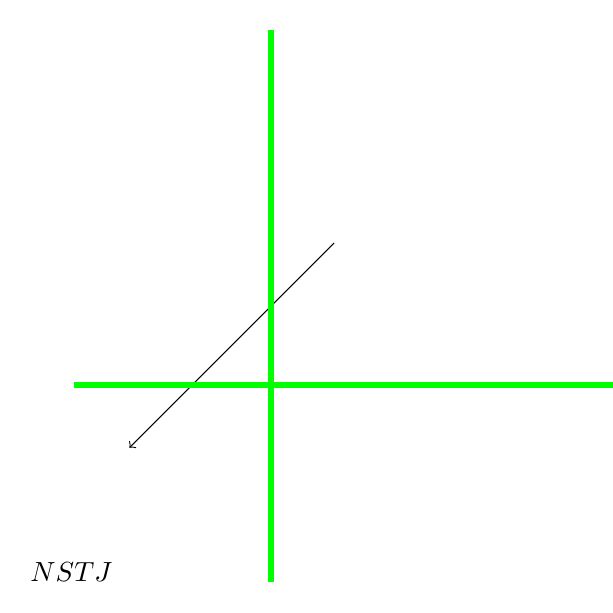
\begin{tikzpicture}
  \creategridjps{9}{7}
  \drawgridnodejps{4}{5}{$N$}
  \drawobstaclejps{7}{7}
  \drawobstaclejps{8}{4}
  \drawobstaclejps{8}{3}
  \drawgridnodejps{1}{2}{$S$}
  \draw[->] (3.3,4.3) -- (0.7,1.7);
  \draw[green,line width=2pt] (0,2.5) -- (7,2.5);
  \draw[green,line width=2pt] (2.5,0) -- (2.5,7);
  \drawgridnodejps{3}{3}{$T$}
  \drawgridnodejps{3}{4}{$J$}
\end{tikzpicture}%
% EOF
